%%%%%%%%%%%%%%%%%%%%%%%%%%%%%%%%%%%%%%%%%%%%%%%%%%%%%%%%%
 % Zawartość tego projektu jest niemodyfikowalna. 
 % Jeżeli chcesz wprowadzić w nim zmiany, to musisz utworzyć jego kopię — patrz https://www.overleaf.com/learn/how-to/Copying_a_project
 %%%%%%%%%%%%%%%%%%%%%%%%%%%%%%%%%%%%%%%%%%%%%%%%%%%%%%%%%
 %
 %	Name			:: 	The official template for the typesetting of diploma theses at the Faculty of Computer Science of AGH University of Krakow
 %	Author			:: 	Stanisław Polak (polak[aT]icsr[DoT]agh[DoT]edu[DoT]pl)
 %	Created			::	2024-02-14
 %	Modified	    ::	2024-03-04
 %	Version			:: 	1.3.1
 %	Email			:: 	polak[aT]icsr[DoT]agh[DoT]edu[DoT]pl
 %	Website			:: 	http://www.icsr.agh.edu.pl/~polak/
 %   Youtube         ::  https://www.youtube.com/user/spolak69
 %   Github          ::  https://github.com/polaksta
 %	License			:: 	This work may be distributed and/or modified under the
 %                       conditions of the LaTeX Project Public License, either version 1.3
 %                       of this license or (at your option) any later version.
 %                       The latest version of this license is in
 %                       http://www.latex-project.org/lppl.txt
 %                       and version 1.3 or later is part of all distributions of LaTeX
 %                       version 2005/12/01 or later.
 %
 %	Description		::	This document is a demonstration of the template
 %
 %%%%%%%%%%%%%%%%%%%%%%%%%%%%%%%%%%%%%%%%%%%%%%%%%%%%%%%%%
 % Niniejszy dokument — szkielet pracy dyplomowej — prezentuje przykłady użycia klasy 'agh-wi' oraz pakietów tradycyjnie używanych w pracach
 % dyplomowych z informatyki. Dla kilku z nich, wartości początkowe parametrów konfiguracyjnych są zdefiniowane 
 % w klasie  — wartości te uwzględniają uwagi osób prowadzących przedmiot "Pracownia Dyplomowa". 
 % Oczywiście możesz używać dowolnych pakietów, niekoniecznie tych, które są pokazane w tym dokumencie
 %%%%%%%%%%%%%%%%%%%%%%%%%%%%%%%%%%%%%%%%%%%%%%%%%%%%%%%%%
 % Poniższe uwagi NIE DOTYCZĄ Overleaf-a
 %%%%%%%%%%%%%%%%%%%%%%%%%%%%%%%%%%%%%%%%%%%%%%%%%%%%%%%%%
 % W tej przykładowej pracy dyplomowej użyto, między innymi, pakietów:
 %   - "minted", co oznacza, że musisz uruchomić kompilator z opcją '-shell-escape'
 %   - "biblatex", co oznacza, że po kompilacji (dokumentu) musisz, jeszcze, wygenerować plik '.bbl'
 %   - "nomencl", co oznacza, że za pomocą komendy 'makeindex' musisz wygenerować wykaz symboli
 %
 % Tak więc, w celu wygenerowania wynikowego dokumentu PDF, musisz wykonać następujące komendy:
 %       pdflatex -shell-escape example
 %       biber example
 %       makeindex example.nlo  -s nomencl.ist -o example.nls
 %       pdflatex -shell-escape example
 %       pdflatex -shell-escape example
 %
 % Dodatkowo musisz mieć zainstalowany program 'pygmentize', który jest częścią pakietu "Pygments" (https://pygments.org/)
 % Ww. programy powinny zainstalować się automatycznie podczas instalacji pakietów LaTeX
 %
 % Jeżeli masz zainstalowany program 'latexmk', to możesz wygenerować dokument PDF następująco:
 %       latexmk example
 %       makeindex example.nlo  -s nomencl.ist -o example.nls
 %       latexmk example
 %
 % Do edycji (oraz komplilacji) dokumentów LaTeX polecam program 'TeXstudio' (https://www.texstudio.org/)
 %
 % Autor: Stanisław Polak <polak[aT]agh[DoT]edu[DoT]pl>
 %%%%%%%%%%%%%%%%%%%%%%%%%%%%%%%%%%%%%%%%%%%%%%%%%%%%%%%%%
 \documentclass[data-science]{agh-wi} % Praca po polsku; na stronie tytułowej, najpierw jest widoczny polskojęzyczny tytuł, a potem angielskojęzyczny.
 % Kierunek 'Informatyka'.
 % Przeznaczona do oglądania przy użyciu przeglądarki PDF.
%%%%%%%%%%%%%%%%%%%%%%%%%%%%%%%%%
% Inne, przykładowe, użycia klasy
%%%%%%%%%%%%%%%%%%%%%%%%%%%%%%%%%
% \documentclass[english]{agh-wi}               % Praca po angielsku; 
                           %     strona tytułowa po polsku, ale najpierw jest widoczny angielskojęzyczny tytuł, a potem polskojęzyczny.  
                           % Kierunek 'Informatyka'.
                           % Przeznaczona do oglądania przy użyciu przeglądarki PDF.
% \documentclass[english, data-science]{agh-wi} % Praca po angielsku; ...
                           % Kierunek 'Informatyka - Data Science'.
                           % Przeznaczona do oglądania przy użyciu przeglądarki PDF.
% \documentclass[print]{agh-wi}                 % Praca po polsku; ...
                           % Kierunek 'Informatyka'.
                           % Przeznaczona do drukowania - każda strona posiada,
                           %    dodatkowy (2cm), margines na oprawę.
%%%%%%%%%%%%%%%%%%%%%%%%%%%%%%%%%%%%%
% Parametry dla strony tytułowej
%%%%%%%%%%%%%%%%%%%%%%%%%%%%%%%%%%%%%
\titlePL{Generacja muzyki przy pomocy dużych modeli językowych}  % Tytuł po polsku
\titleEN{Music generation with Lange Language Models} % Tytuł po angielsku
\author{Filip Ręka}
\supervisor{dr hab. Maciej Smołka prof. AGH}
%%%%%%%%%%%%%%%%%%%%%%%%%%%%%%%%%%%%%
% Pakiety
%%%%%%%%%%%%%%%%%%%%%%%%%%%%%%%%%%%%%
% Podstawowe — na pewno będziesz ich potrzebował(a) w swojej wersji pracy dyplomowej
%%%%%%%%%%%%%%%%%%%%%%%%%%%%%%%%%%%%%
\usepackage{polski} % Obsługa języka polskiego
%%%%%%%%%%%%%%%%%%%%%%%%%%%%%%%%%%%%%
% Dodatkowe — niekoniecznie będziesz ich potrzebował(a) w swojej wersji pracy dyplomowej
%%%%%%%%%%%%%%%%%%%%%%%%%%%%%%%%%%%%%
\usepackage[sorting=none]{biblatex}           % Spis literatury ma być tworzony na podstawie zawartości bibliograficznej bazy danych
\usepackage{amsmath}                          % Dodatkowe środowiska matematyczne
\usepackage{amssymb}                          % Dodatkowe symbole matematyczne
\usepackage[polish, intoc]{nomencl}           % Definiowanie symboli
\usepackage{graphicx}                         % Wstawianie grafik zewnętrznych
\usepackage{xcolor}                           % Kolorowy tekst
\usepackage{tabularx}                         % Rozszerzona wersja środowiska 'tabular'
\usepackage{longtable}                        % Skład "długich" tabel
\usepackage[ruled,linesnumbered]{algorithm2e} % Algorytmy w formie pseudokodu
\usepackage{listings}                         % Formatowanie kodów źródłowych programów
\usepackage[newfloat]{minted}                 % Formatowanie kodów źródłowych programów
\usepackage{hyperref}                         % Obsługa adresów URL — zbędny jeżeli używasz 'biblatex'
\usepackage{csquotes}                         % Polskie cudzysłowy — rekomendowany jeżeli używasz 'biblatex'
\usepackage{tocloft}
%%%%%%%%%%%%%%%%%%%%%%%%%%%%%%%%%%%%
%  % Konfiguracja rysunków TikZ
%%%%%%%%%%%%%%%%%%%%%%%%%%%%%%%%%%%%
\usetikzlibrary{shapes.geometric,arrows.meta} 
\tikzstyle{every picture}+=[remember picture]
\tikzstyle{na} = [baseline=-.5ex]
%%%%%%%%%%%%%%%%%%%%%%%%%%%%%%%%%%%%
% Ładowanie danych bibliograficznych
%%%%%%%%%%%%%%%%%%%%%%%%%%%%%%%%%%%%
\addbibresource{bibliography.bib}
%%%%%%%%%%%%%%%%%%%%%%%%%%%%%%%%%%%%%
% Opcje konfiguracyjne pakietów
%%%%%%%%%%%%%%%%%%%%%%%%%%%%%%%%%%%%%
% Pakiet 'framed'
\definecolor{shadecolor}{gray}{0.9}
% Pakiet 'nomencl'
\makenomenclature % Otwórz plik 'example.nlo'
%%%%%%%%%%%%%%%%%%%%%%%%%%%%%%%%%%%%%
% Definicje komend
%%%%%%%%%%%%%%%%%%%%%%%%%%%%%%%%%%%%%
\newcommand{\alert}[1]{\colorbox{red!50}{#1}}
%%%%%%%%%%%%%%%%%%%%%%%%%%%%%%%%%%%%%
% Twierdzenia i podobne struktury
%%%%%%%%%%%%%%%%%%%%%%%%%%%%%%%%%%%%%
\newtheorem{theorem}{Twierdzenie}
\newtheorem{definition}{Definicja}

%%%%%%%%%%%%%%%%%%%%%%%%%%%%%%%%%%%%%
% Ustawienie licznika do subsubsection
%%%%%%%%%%%%%%%%%%%%%%%%%%%%%%%%%%%%%
\setcounter{secnumdepth}{5}

\newcounter{comment}[chapter]
\newenvironment{comment}[1][]{\begin{shaded}\refstepcounter{comment}
\noindent \textbf{Uwaga~\thechapter.\thecomment. #1} \rmfamily}{\end{shaded}}
%%%%%%%%%%%%%%%%%%%%%%%%%%%%%%%%%%%%%
%%%%%%%%%%%%%%%%%%%%%%%%%%%%%%%%%%%%%
\begin{document}
%%%%%%%%%%%%%%%%%%%%%%%%%%%%%%%%%%%%%
\frontmatter % Część wstępna
%%%%%%%%%%%%%%%%%%%%%%%%%%%%%%%%%%%%%
\maketitle % Dodaj stronę tytułową
%%%%%%%%%%%%%%%%%%%%%%%
% Jeżeli chcesz komuś podziękować, to możesz użyć poniższego kodu
\cleardoublepage
\thispagestyle{empty}
\vspace*{\fill}
\begin{flushright}
    \em
    \begin{minipage}{0.75\textwidth}
        Tutaj możesz umieścić treść podziękowań.
        Tutaj możesz umieścić treść podziękowań.
        Tutaj możesz umieścić treść podziękowań.
        Tutaj możesz umieścić treść podziękowań.
        Tutaj możesz umieścić treść podziękowań.
    \end{minipage}
\end{flushright}
%%%%%%%%%%%%%%%%%%%%%%%
\begin{abstractPL}
    Duże modele językowe (ang. \textit{Large Language Models} \textbf{LLM}) charakteryzują się zdolnością do generacji języka oraz innych zadań w przetwarzania języka naturalnego, takich jak na przykład klasyfikacja. Zdolność tą nabierają podczas czasochłonnego oraz intensywnego obliczeniowego treningu metodami samo odraz pół-nadzorowanego, podczas którego uczą się one relacji z wielkiej ilości dokumentów tekstowych. LLMy mogą zostać wykorzystane do generacji tekstu, formy generatywnej sztucznej inteligencji, poprzez pobieranie tekstu wejściowego i wielokrotne przewidywanie kolejnego tokenu lub słowa w tekście. Strukturę muzyki można porównać struktury tekstu pisanego, gdzie każda nuta odpowiada literze lub słowu, akordy zdaniom a dłuższe i sekwencję paragrafom. Poniższa praca, zamierza zbadać możliwości generacyjne LLMów wytrenowanych na muzycznych zbiorach danych.
\end{abstractPL}
\begin{abstractEN}
    Abstract in English \cite{attention} \ldots
\end{abstractEN}
%%%%%%%%%%%%%%%%%%%%%%%%%%%%%%%%%%%%%
%%%%%%%%%%%%%%%%%%%%%%%%%%%%%%%%%%%%%
% \setlength{\cftsecnumwidth}{4em} % Adjust according to your needs
% \setlength{\cftsubsubsecindent}{8em} % Adjust according to your needs
\setcounter{tocdepth}{5}
\tableofcontents{5}   % Wygeneruj spis treści

\begin{shaded}
    Zawartość spisu treści \pauza tytuły rozdziałów oraz ich liczba zależą od tematyki pracy \pauza należy ustalić z opiekunem pracy.
\end{shaded}
\listoffigures     % Wygeneruj listę rysunków
\listoftables      % Wygeneruj listę tabel
\listofalgorithms  % Wygeneruj listę algorytmów
% Wygeneruj listę kodów źródłowych
\lstlistoflistings % Jeżeli do tworzenia listingów używasz pakietu 'listings'
%  \listoflistings % Jeżeli do tworzenia listingów używasz pakietu 'minted'
\printnomenclature % Wyświetl listę symboli
%%%%%%%%%%%%%%%%%%%%%%%%%%%%%%%%%%%%%
\mainmatter % Część główna
%%%%%%%%%%%%%%%%%%%%%%%%%%%%%%%%%%%%%
\chapter{Wstęp}
\begin{comment}
Tytuł oraz strukturę rozdziału należy ustalić z opiekunem pracy.
\end{comment}
Wprowadzenie w tematykę pracy.
\section{Cel i zakres pracy}
Streszczenie specyfikacji wymagań Promotora.
\chapter{Część literaturowa}

\section{Cyfrowa reprezentacja muzyki}

\subsection{WAV (ang. \textit{waveform audio format})}

\subsection{MIDI (ang. \textit{Musical Instrument Digital Interface})}

\subsection{Podobieństwa reprezentacji muzyki oraz tekstu}

\subsection{Tokenizacja}
\cite{miditok2021}

\section{Zbiory danych}

\subsection{Johann Sebastian Bach Chorales}
Datset \cite{bachchorales}

\subsection{The MAESTRO v3.0}
Dataset \cite{maestrov3}

\subsection{Million Song Dataset}
Dataset i takie cytowanko \cite{milionsongs}

\section{STOA}
Tutaj nie wiem do końca w jakiej kolejności chciałbym o tym pisać, ponieważ z jednej strony przedstawienie STOA przed czymkolwiek jest ok, ale nie chciałbym pisać o czymś czego jeszcze w pracy nie wprowadziłem.

\section{Architekturze transformera}
\subsection{Algorytm uwagi (ang. \textit{attention})}
\subsection{Warianty mechanizmu uwagi}
\subsubsection{Self attention}
\subsubsection{Multi-headed attention}
\subsubsection{Flash attention}
\subsection{Budowa transformera}
\begin{figure}[!ht]
    \begin{center}
        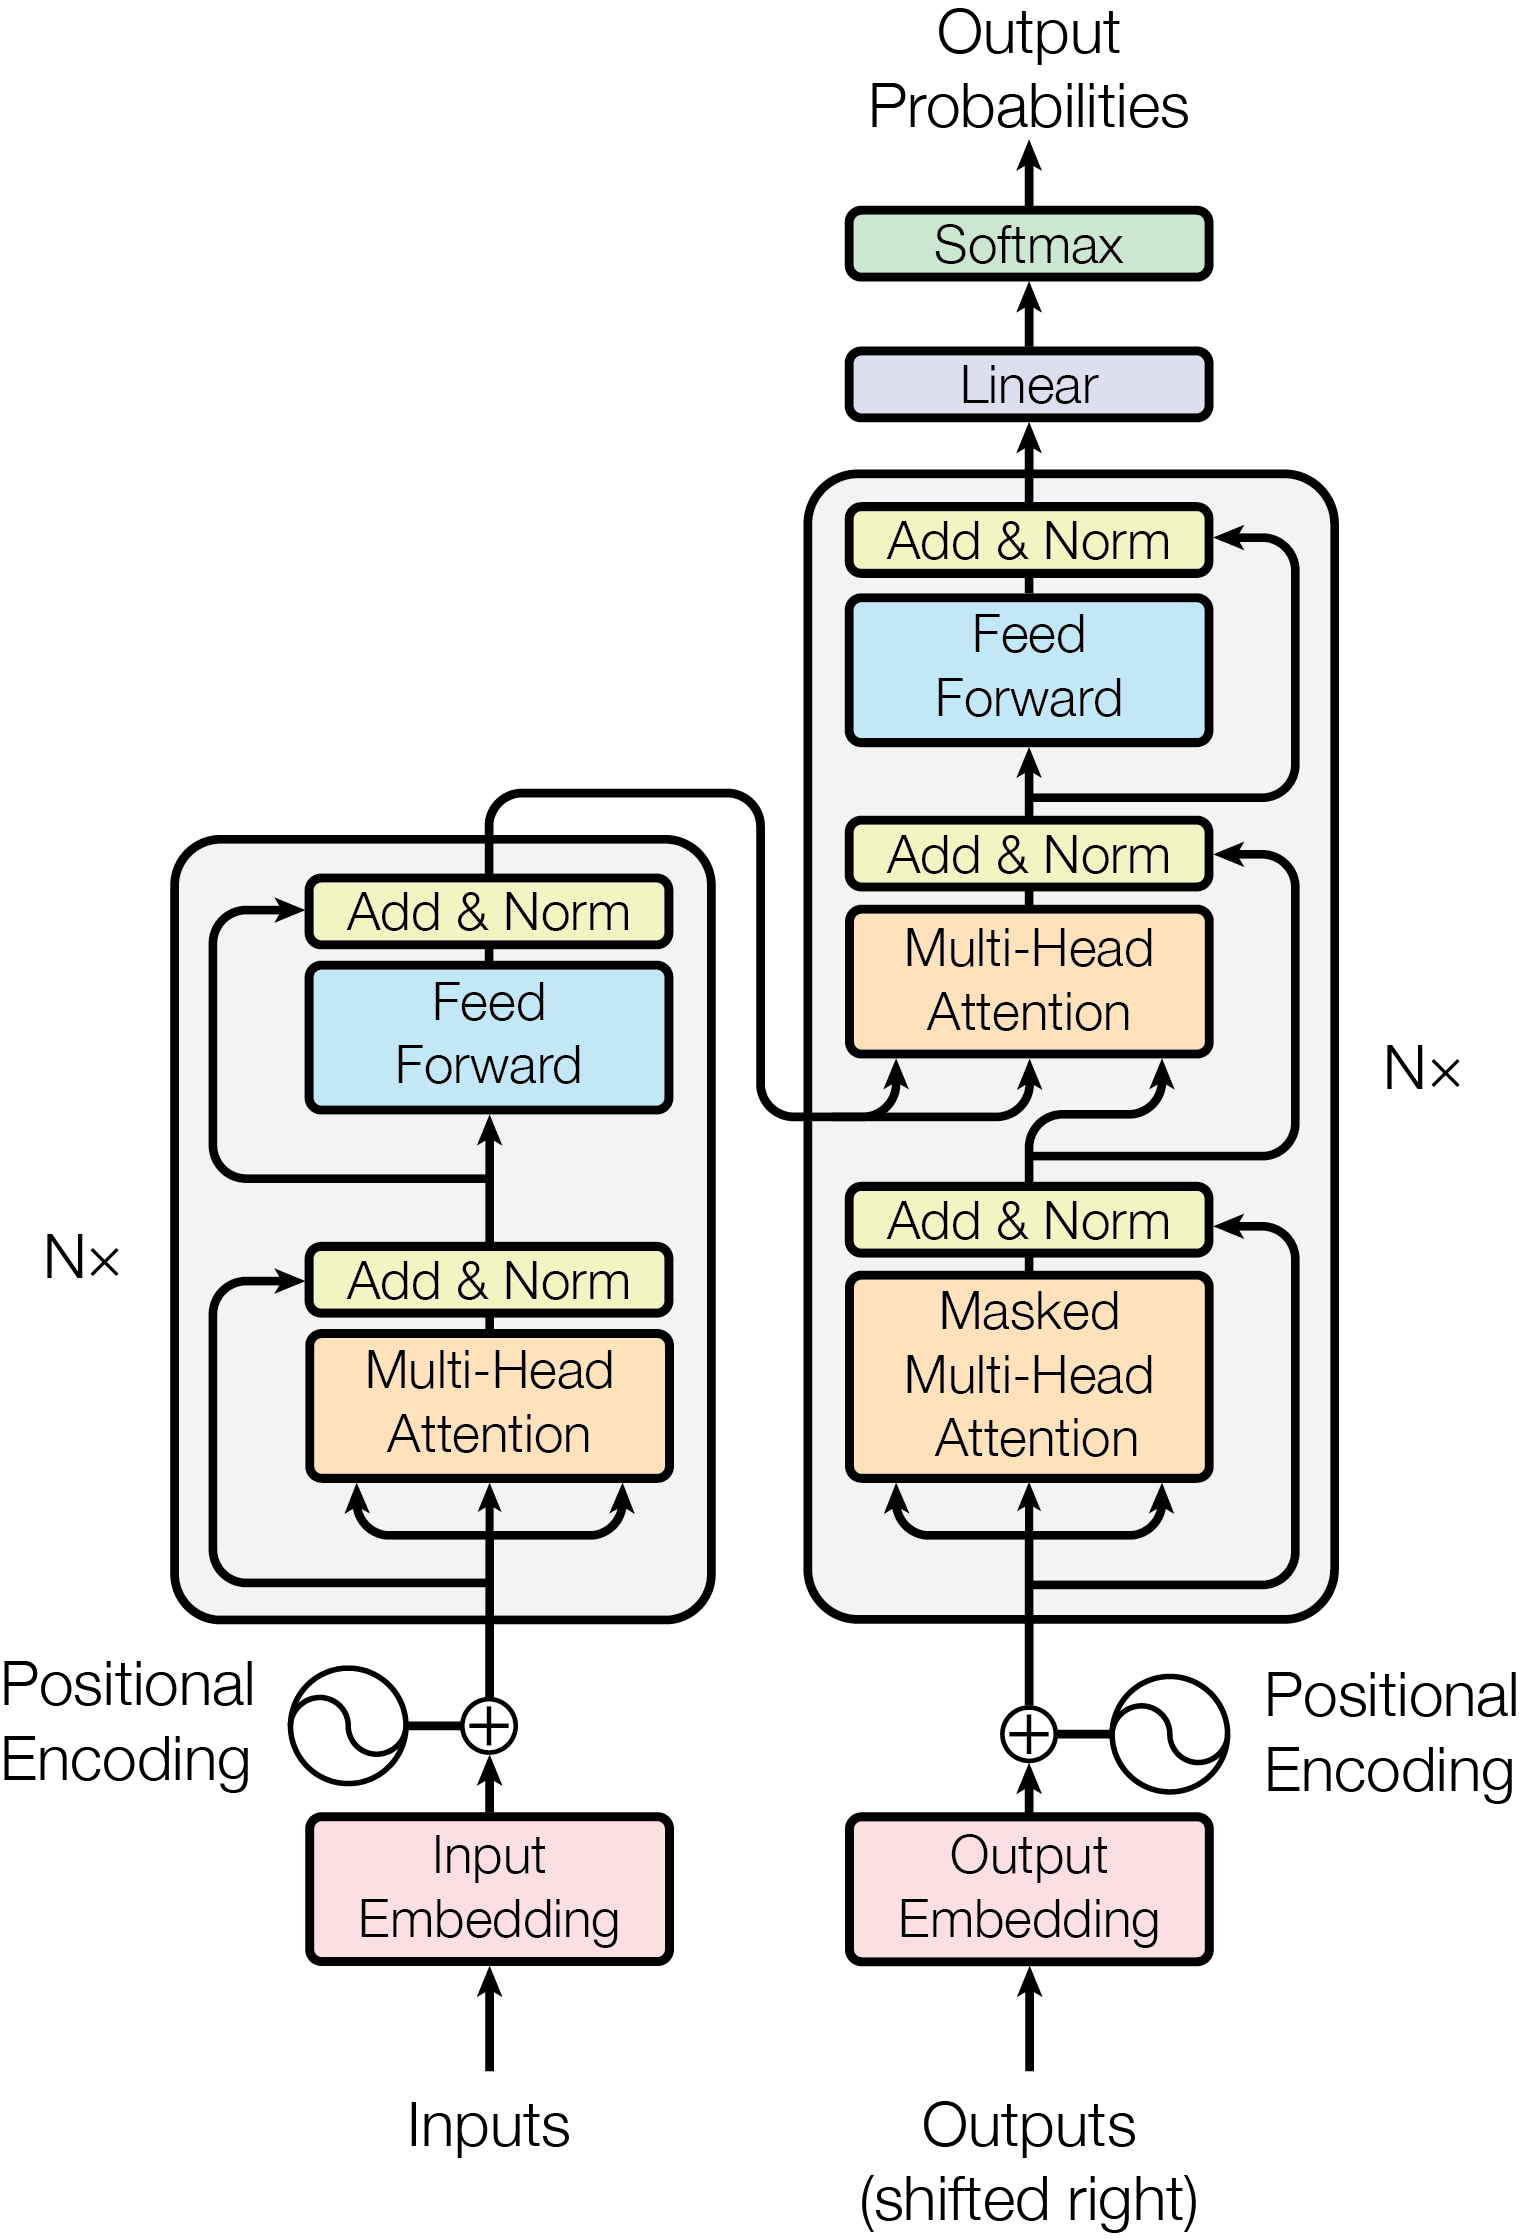
\includegraphics[width=0.7\linewidth]{img/transformer1}
    \end{center}
    \caption{Schemat transformera.}
    \label{fig:transformer1}
\end{figure}
\subsection{Modele tranformerowe}
\subsubsection{\textit{Classic} transformer}
\subsubsection{SeqGAN}
\subsubsection{Mistral}

\section{Architektura \textit{state space}}
\subsection{Mamba}
\subsection{Tutaj się rozdrobnić trzeba}
\begin{figure}
    \begin{center}
        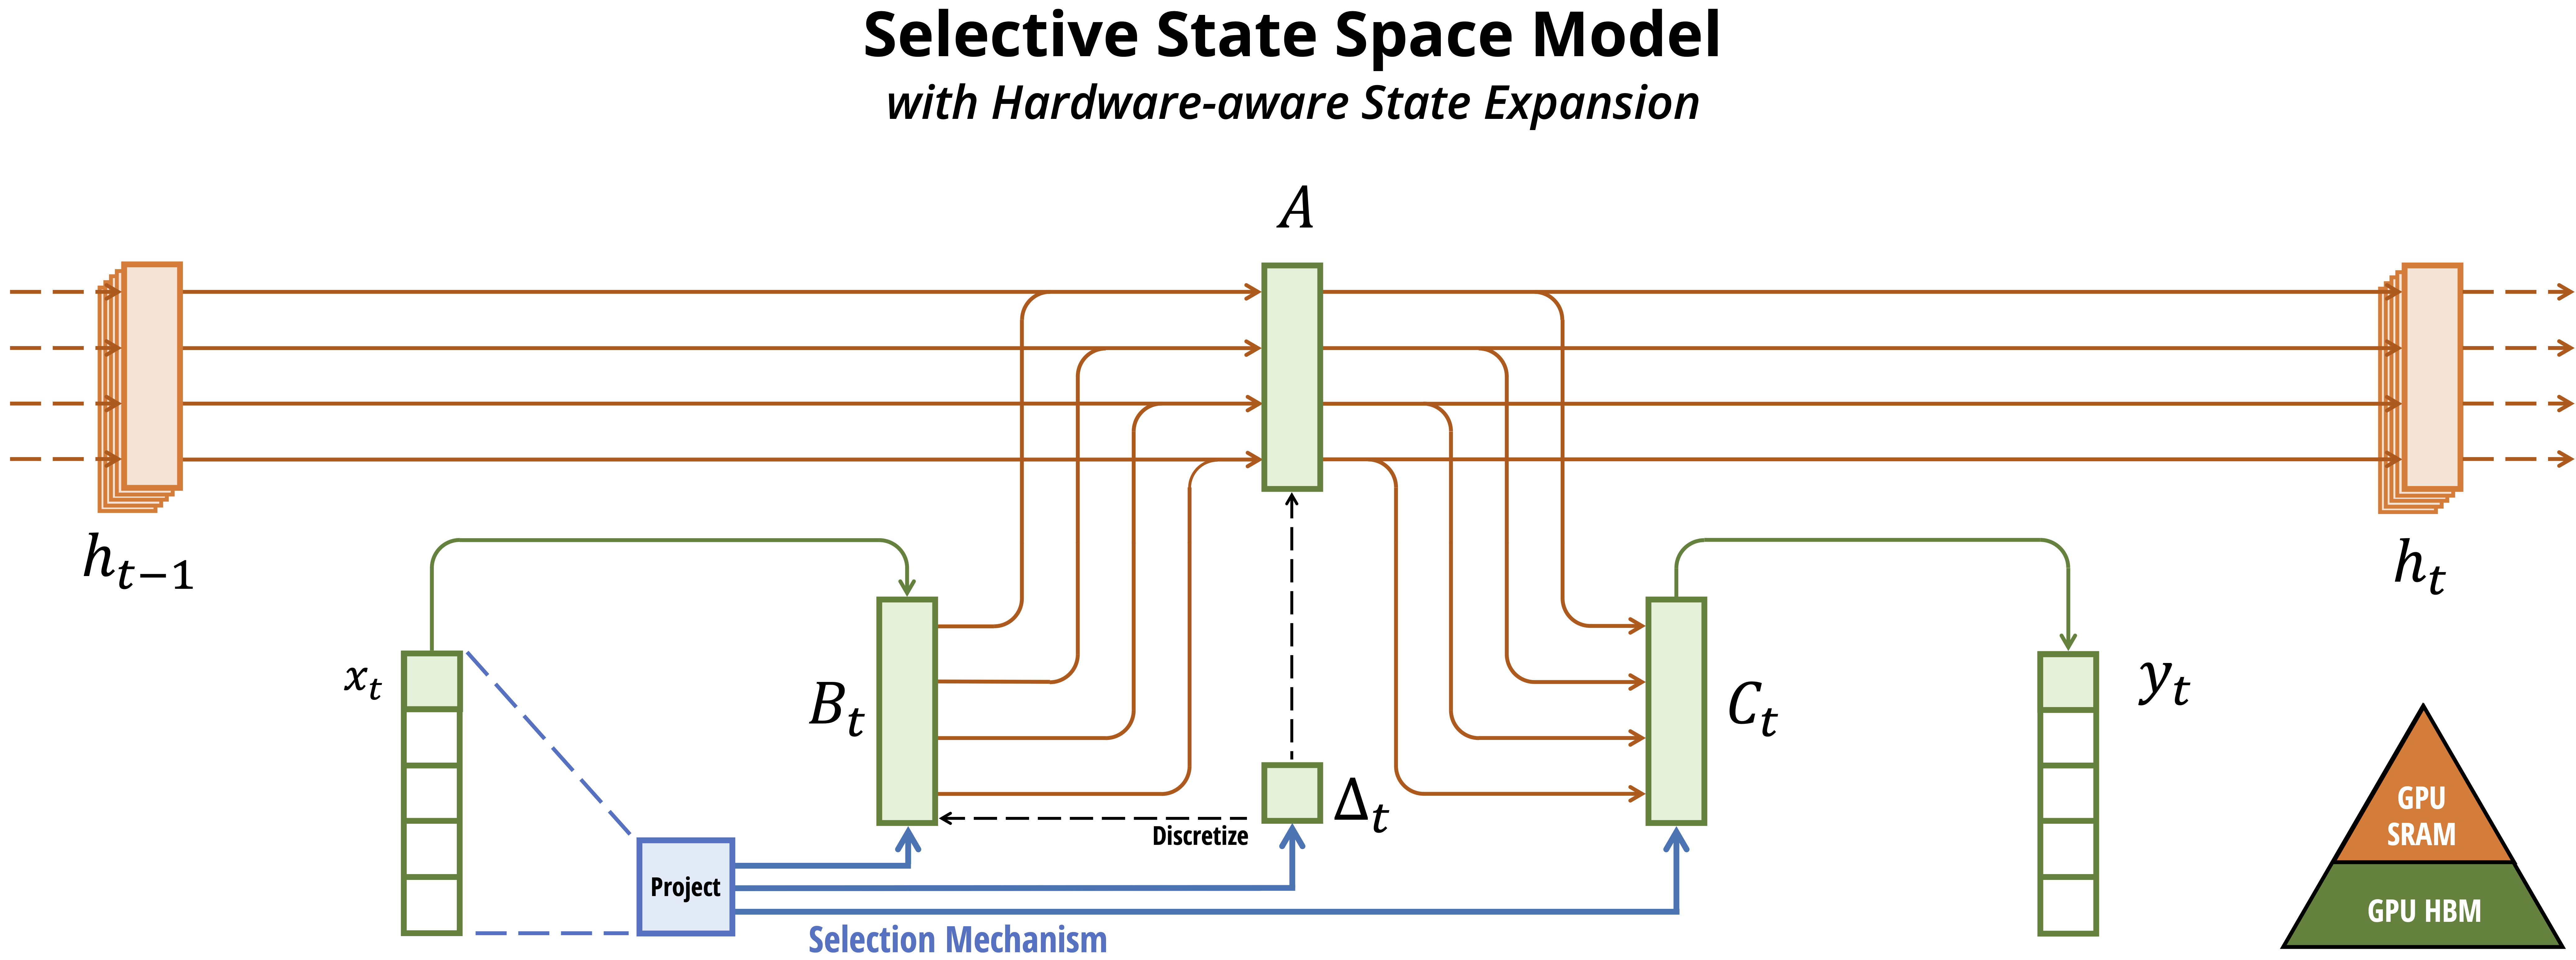
\includegraphics[width=0.9\linewidth]{img/mamba1.png}
    \end{center}
    \caption{Schemat modelu Mamba.}
    \label{fig:mamba1}
\end{figure}

\begin{comment}
Tytuł oraz strukturę rozdziału należy ustalić z opiekunem pracy.
\end{comment}

Aktualny stan wiedzy, na dany temat, na podstawie dostępnej literatury naukowej oraz specjalistycznej.
\chapter{Część badawcza}
\begin{comment}
Tytuł oraz strukturę rozdziału należy ustalić z opiekunem pracy.
\end{comment}
\section{Opis \textit{pipeline-u}}
Tutaj zamierzam opisać w jaki sposób modele zostały stworzone, jakie bilbioteki zostały użyte, jaki sprzęto został użyty podczas treningu
\section{Porównanie architektur użytych modeli}
\section{Prezentacja otrzymanych wyników}
\section{Porównanie wyników}
Celem porównania otrzymanych wyników z dowolnych modeli, jest ocena jakości ich pracy. W kontekście modeli dyskryminujących (ang. \textit{discriminative model}), na przykład klasyfikatorów bądź modeli regresyjnych, ocena ich jakości jest dość prosta, ponieważ istnieje predefiniowana, prawdziwa wartość w zbiorze testowym, którą model próbuje przewidzieć. W takim przypadku ewaluacja jakości modelu to porównanie prawdziwych danych, z tymi przewidzianymi przez model. Porównanie odbywa się przez policzenie metryk np. dla modelu klasyfikującego celności, precyzji, \textit{F1-score} lub dla modelu regresyjnego MSE lub $R^2$. W przypadku modeli generacyjnych celem treningu jest jak najlepsza aproksymacja rozkładu prawdopodobieństwa danych $P(X_{data})$ lub w przypadku danych oznaczonych łączny rozkład $P(X, Y)$. W przypadku dużej wymiarowości danych, obliczenie obiektywnych metryk takich jak \textit{log-likelihood} lub dywergencja Kullbacka-Leiblera (\textit{KLD}) często jest nieobliczalne. Dla człowieka weryfikacja wyników modeli generacyjnych takich jak \textit{text-to-speech} lub \textit{text-to-image} jest trywialnym zadaniem, jednak nie jest to oczywiste zadanie algorytmiczne. Często odwołuje się do subiektywnych metryk takich jak \textit{MOS ang. mean opinion score}, które oblicza się jako średnią opinię np. w skali od 1-5 braną z zazwyczaj niewielkiej grupy ludzi. Niestety metryka ta często nie jest wiarygodna ze względu na jej subiektywności niewielką próbę badawczą. Aby wyeliminować te wady serwisy takie jak \textit{HuggingFace} udostępniają narzędzia dla członków społeczności, które pozwalają na ranking modeli, z nadzieją że zgodnie z prawem wielkich liczb, przy wystarczającej liczbie odpowiedzi, uda się otrzymać w miarę obiektywną ocenę. Przykładowym narzędziem tego rodzaju jest \textit{The TTS Arena}\cite{tts_arena}, która pozwala na ranking modeli \textit{text-to-speech}.

W przypadku muzyki, istnieje możliwość aby zweryfikować poprawność wygenerowanych sekwencji odwołując się do teorii oraz harmonii muzyki. Istnieje kilka narzędzi takich jak \textit{Chordify}, \textit{Hooktheory} lub \textit{Sibelius}, które pozwalają na analizę harmoniczną utworów, dzieki czemu autorzy mogą w prosty sposób analizować i dobierać progresję danej melodii. Niestety większość takich narzędzi jest płatna i nie pozwala na zautomatyzowaną analizę wielu plików. Dodatkowym problemem jest w analizie harmonicznej, szczególnie prowadzonej przez algorytmy, jest rozróżnienie harmonii wertykalnej oraz horyzontalnej. Rozróżnienie to zostało wytłumaczone przez Jacoba Colliera, kilkukrotnego laureata nagród \textit{Grammy}, którego zdaniem akord, który nawet zagrany sam brzmi niepoprawnie, w odpowiednim kontekście i przez odpowiednią progresję w kolejnych fragmentach muzyki, może mieć nadany sens, przez co cała sekwencja nabiera muzycznego piękna\cite{collier_wrongnote}.
\begin{comment}
W mojej pracy prawdopodobnie zostanie zastosowane podejście MOS dla dość niewielkiej grupy ludzi, jednak jeśli triale oprogramowania pozwola, spróbuję przynajmniej sprawdzić czy taka analiza pozwala na jakieś sensowne obliczenie metryki
\end{comment}
\chapter{Zakończenie}
\begin{comment}
Tytuł oraz strukturę rozdziału należy ustalić z opiekunem pracy.
\end{comment}
\begin{enumerate}
    \item Podsumowanie.
    \item Możliwości dalszego rozwoju.
    \item Potencjalne obszary zastosowania pracy.
\end{enumerate}
%%%%%%%%%%%%%%%%%%%%%%%%%%%%%%%%%%%%%
%%%%%%%%%%%%%%%%%%%%%%%%%%%%%%%%%%%%%
\appendix % Dodatek
\chapter{Typowe elementy składowe pracy dyplomowej z informatyki}
\section{Tabele}
\begin{comment}
\begin{itemize}
    \item Każda tabela powinna być opisana w treści pracy.
    \item Podpis ma być przed tabelą.
\end{itemize}
\end{comment}
W tabeli \ref{tab:result} przedstawiono wyniki pomiarów.
\begin{table}[!h]
    \caption{Pomiary zużycia energii elektrycznej\label{tab:result}.}
    \centering
    \begin{tabular}{|l||r@{,}l|}
        \hline
        \textbf{L.p.} & \multicolumn{2}{|c|}{\textbf{Wartość}}          \\
        \hline
        \hline
        \cline{2-3}
        %\textbf{L.p.} & \multicolumn{1}{r@{\,\vline\,}}{Całkowita} & Ułamkowa \\
        \hline
        1             & 12345                                  & 6789   \\
        \cline{2-3}
                      & 45                                     & 89     \\
        \hline
        2             & 45                                     & 678901 \\
        \hline
    \end{tabular}
\end{table}

Jeżeli tabela zawiera dużą liczbę wierszy i może nie zmieścić się na stronie \pauza patrz tabela \ref{tab:longtable} \pauza skorzystaj z pakietu \emph{longtable} \cite{longtable}.
\begin{longtable}{|p{14ex}|p{1.5em}|p{1.5em}|p{1.5em}|p{1.5em}|p{1.5em}|p{1.5em}|p{1.5em}|p{1.5em}|p{1.5em}|}
    \caption{Tabela, która zawiera dużą liczbę wierszy\label{tab:longtable}.}
    \endfirsthead
    \hline
              & 1 & 2 & 3 & 4 & 5 & 6 & 7 & 8 & \\
    \cline{2-9}
              &   &   &   &   &   &   &   &   & \\
    \hline
    \endhead
    \endfoot
    \hline\hline
              & 1 & 2 & 3 & 4 & 5 & 6 & 7 & 8 & \\
    \cline{2-9}
              &   &   &   &   &   &   &   &   & \\
    \hline\hline
    Student 1 &   &   &   &   &   &   &   &   & \\
    \cline{2-9}
              &   &   &   &   &   &   &   &   & \\
    \hline\hline
    Student 2 &   &   &   &   &   &   &   &   & \\
    \cline{2-9}
              &   &   &   &   &   &   &   &   & \\
    \hline\hline
    Student 3 &   &   &   &   &   &   &   &   & \\
    \cline{2-9}
              &   &   &   &   &   &   &   &   & \\
    \hline\hline
    Student 4 &   &   &   &   &   &   &   &   & \\
    \cline{2-9}
              &   &   &   &   &   &   &   &   & \\
    \hline\hline
    Student 5 &   &   &   &   &   &   &   &   & \\
    \cline{2-9}
              &   &   &   &   &   &   &   &   & \\
    \hline\hline
    Student 6 &   &   &   &   &   &   &   &   & \\
    \cline{2-9}
              &   &   &   &   &   &   &   &   & \\
    \hline\hline
    Student 7 &   &   &   &   &   &   &   &   & \\
    \cline{2-9}
              &   &   &   &   &   &   &   &   & \\
    \hline\hline
    Student 8 &   &   &   &   &   &   &   &   & \\
    \cline{2-9}
              &   &   &   &   &   &   &   &   & \\
    \hline\hline
    Student 9 &   &   &   &   &   &   &   &   & \\
    \cline{2-9}
              &   &   &   &   &   &   &   &   & \\
    \hline\hline
    % Student 10 &   &   &   &   &   &   &   &   & \\
    % \cline{2-9}
    %            &   &   &   &   &   &   &   &   & \\
    % \hline\hline
    % Student 11 &   &   &   &   &   &   &   &   & \\
    % \cline{2-9}
    %            &   &   &   &   &   &   &   &   & \\
    % \hline\hline
    % Student 12 &   &   &   &   &   &   &   &   & \\
    % \cline{2-9}
    %            &   &   &   &   &   &   &   &   & \\
    % \hline\hline
    % Student 13 &   &   &   &   &   &   &   &   & \\
    % \cline{2-9}
    %            &   &   &   &   &   &   &   &   & \\
    % \hline\hline
\end{longtable}

Tabele, w których występuje długi tekst, a co za tym idzie może się on nie zmieścić \pauza musi zostać zawinięty, z pomocą przychodzi środowisko 'tabularx' \cite{tabularx} \pauza  patrz tabela \ref{tab:tabularx}.
\begin{table}[!ht]
    \caption{Tabela zawierająca długi tekst\label{tab:tabularx}.}
    \centering
    \begin{tabularx}{300pt}{|c|X|c|X|}
        \hline
        \multicolumn{2}{|c|}{Wpis wielokolumnowy!} &
        TRZY                                       &
        CZTERY                                       \\
        \hline
        jeden                                      &
        \raggedright\arraybackslash Szerokość tej kolumny zależy od
        szerokości tabeli.                         &
        trzy                                       &
        \raggedright\arraybackslash Kolumna czwarta będzie zachowywać się w taki sam sposób jak
        druga kolumna o tej samej szerokości.        \\
        \hline
    \end{tabularx}
\end{table}
%%%%%%%%%%%%%%%%%%%%%%%%%%%%%%%%%%%%%
\section{Rysunki}
\begin{comment}
\begin{itemize}
    \item Rysunki powinny być przerysowane samodzielnie albo używane tylko te,
          których twórcy zezwolili na ich rozpowszechnianie oraz kopiowanie, czyli
          np. rysunki objęte licencją Creative Commons.
    \item Każdy rysunek powinien być opisany w treści pracy.
\end{itemize}
\end{comment}
\subsection{Wewnętrzne}
Klasa \emph{agh-wi}, automatycznie, dołącza pakiet \emph{TikZ} \cite{tikz} \pauza dostarcza on komend pozwalających na tworzenie grafik. Przykładowe grafiki pokazano na rysunku \ref{fig:tikz1} oraz \ref{fig:tikz2}.
%%%%%%%%%%%%%%%%%
\begin{figure}[!h]
    \begin{center}
        \tikz \draw[thick,rounded corners=8pt]
        (0,0) -- (0,2) -- (1,3.25) -- (2,2) -- (2,0) -- (0,2) -- (2,2) -- (0,0) -- (2,0);
    \end{center}
    \caption{Prosty rysunek \emph{TikZ}\label{fig:tikz1}.}
\end{figure}
%%%%%%%%%%%%%%%%%
\begin{figure}[!ht]
    \begin{center}
        \begin{tikzpicture}
            \draw[step=.5cm,gray,very thin] (-1.4,-1.4) grid (1.4,1.4);
            \draw (-1.5,0) -- (1.5,0);
            \draw (0,-1.5) -- (0,1.5);
            \draw (0,0) circle [radius=1cm];
        \end{tikzpicture}
    \end{center}
    \caption{Bardziej złożony rysunek \emph{TikZ}\label{fig:tikz2}.}
\end{figure}
%%%%%%%%%%%%%%%%%

Oprócz rysunków eksponowanych możliwe jest tworzenie grafik będących  \tikz{\fill[orange] (0ex,0ex) circle (1ex);  \fill[red] (1ex,1ex) circle (1ex);} częścią \tikz{\draw (0pt,0pt) -- (20pt,6pt);} zdania.

\emph{TikZ} pozwala również na kreślenie po powierzchni strony, np. możemy narysować strzałki pomiędzy elementami strony.
\begin{shaded}
    %%%%%%%%%%%%%%%%%%%%%%%%%%%%%%%%%%%%%%%%%%%%%%%%%%%
    % Zmodyfikowana wersja przykładu ze strony  https://texample.net/tikz/examples/global-nodes/
    %%%%%%%%%%%%%%%%%%%%%%%%%%%%%%%%%%%%%%%%%%%%%%%%%%%
    Ułamek \pauza patrz wzór \ref{eqn:tikz} \pauza składa się z:
    \begin{itemize}
        \item Licznika \tikz[na] \node (n1) {};
    \end{itemize}
    %%%%%%%%%%%%%%%%%
    \begin{equation}
        a =  \frac{\tikz[baseline] \node[fill=blue!20,rectangle] (t1){$x+y$};}{\tikz[baseline] \node[fill=red!20, ellipse] (t2){$y-z$}; }
        \label{eqn:tikz}
    \end{equation}
    %%%%%%%%%%%%%%%%%
    \begin{itemize}
        \item Mianownika \tikz\node[na] (n2) {};
    \end{itemize}
    %%%%%%%%%%%%%%%%%
    \begin{tikzpicture}[overlay]
        \path  (n1) edge [->,bend left] (t1);
        \path  (n2) edge [->,bend right] (t2);
    \end{tikzpicture}
\end{shaded}
\subsection{Zewnętrzne}
Oczywiście możliwe jest również dołączanie rysunków zewnętrznych \pauza
pakiet \emph{graphicx} \cite{graphicx} pozwala na wstawianie grafik zapisanych w  plikach: '.png', '.jpg' oraz '.pdf'. Rysunek \ref{fig:logo} wstawiono przy użyciu tego pakietu.
\begin{figure}[!ht]
    \begin{center}
        \IfFileExists{img/logo_podstawowe.png}{
            
\includegraphics[width=0.7\linewidth]{img/logo_podstawowe}
        }
        {Nie znaleziono pliku 'img/logo\_podstawowe.png' \pauza pobierz go ze strony \url{https://www.informatyka.agh.edu.pl/media/uploads/Logo WI/PNG/logo_podstawowe.png}}
    \end{center}
    \caption{Logo Wydziału Informatyki.}
    \label{fig:logo}
\end{figure}
%%%%%%%%%%%%%%%%%%%%%%%%%%%%%%%%%%%%%
\section{Kody źródłowe}
Najpopularniejszymi pakietami, które umożliwiają składanie kodów źródłowych programów, są:
\begin{description}
    \item[listings \cite{listings}] \pauza kod źródłowy jest formatowany bezpośrednio przez \LaTeX{}\dywiz{}a \pauza nie jest używany żaden, zewnętrzny, formater kodu.
        \begin{lstlisting}[language=C++, float=ht, label=lst:code1, caption={Przykładowy kod źródłowy sformatowany za pomocą pakietu 'listings'.}]
/* Pierwszy program w C++ */

#include <iostream>

int main() {
std::cout << "Hello World!";
return 0;
}
\end{lstlisting}
    \item[minted \cite{minted}] \pauza formatuje kod źródłowy przy użyciu biblioteki języka Python  o nazwie \emph{Pygments} \cite{pygments}.
        \begin{listing}[!ht]
            \caption{Przykładowy listing sformatowany za pomocą pakietu 'minted'.\label{lst:code2}}
            \begin{minted}{c++}
/* Pierwszy program w C++ */

#include <iostream>

int main() {
std::cout << "Hello World!";
return 0;
}
\end{minted}
        \end{listing}
\end{description}

\begin{comment}
\begin{itemize}
    \item Podpis ma być przed kodem źródłowym.
    \item \alert{Proszę używać tylko jednego z tych pakietów}; w przeciwnym razie otrzymasz taki efekt, jak w przykładowej pracy \pauza obydwa listingi mają ten sam numer.
\end{itemize}
\end{comment}

Kod źródłowy w C++ sformatowany przy użyciu pakietu \emph{listings}, pokazano na listingu \ref{lst:code1}; sformatowany przy użyciu pakietu \emph{minted}, pokazano na listingu \ref{lst:code2}.
%%%%%%%%%%%%%%%%%%%%%%%%%%%%%%%%%%%%%
\section{Algorytmy}
Pakiet \emph{algorithm2e} \cite{algorithm2e} to jeden z kilku, które pozwalają zapisywać algorytmy w formie pseudokodu \pauza patrz
algorytm \ref{alg:algo_disjdecomp}.
\begin{comment}
Podpis ma być przed algorytmem.
\end{comment}
\begin{algorithm}[!htb]
    \caption{Disjoint decomposition.}\label{alg:algo_disjdecomp}
    %%%%%%%%%%%%%%%%%%%%%%%%%%     
    \SetKwData{Left}{left}\SetKwData{This}{this}\SetKwData{Up}{up}
    \SetKwFunction{Union}{Union}\SetKwFunction{FindCompress}{FindCompress}
    \SetKwInOut{Input}{input}\SetKwInOut{Output}{output}
    \Input{A bitmap $Im$ of size $w\times l$}
    \Output{A partition of the bitmap}
    \BlankLine
    \emph{special treatment of the first line}\;
    \For{$i\leftarrow 2$ \KwTo $l$}{
        \emph{special treatment of the first element of line $i$}\;
        \For{$j\leftarrow 2$ \KwTo $w$}{\label{forins}
            \Left$\leftarrow$ \FindCompress{$Im[i,j-1]$}\;
            \Up$\leftarrow$ \FindCompress{$Im[i-1,]$}\;
            \This$\leftarrow$ \FindCompress{$Im[i,j]$}\;
            \If(\tcp*[h]{O(\Left,\This)==1}){\Left compatible with \This}{\label{lt}
                \lIf{\Left $<$ \This}{\Union{\Left,\This}}
                \lElse{\Union{\This,\Left}}
            }
            \If(\tcp*[f]{O(\Up,\This)==1}){\Up compatible with \This}{\label{ut}
                \lIf{\Up $<$ \This}{\Union{\Up,\This}}
                \tcp{\This is put under \Up to keep tree as flat as possible}\label{cmt}
                \lElse{\Union{\This,\Up}}\tcp*[h]{\This linked to \Up}\label{lelse}
            }
        }
        \lForEach{element $e$ of the line $i$}{\FindCompress{p}}
    }
\end{algorithm}\DecMargin{1em}
%%%%%%%%%%%%%%%%%%%%%%%%%%%%%%%%%%%%%
\section{Wzory}
\LaTeX{} bardzo dobrze sprawdza się w przypadku prac dyplomowych zawierających wzory matematyczne\footnote{ W przypadku złożonych wzorów warto zastosować pakiet \emph{amsmath} \cite{amsmath}.}.
\subsection{Przykłady}
Wzór $E = mc^{2}$\nomenclature{$c$}{Prędkość światła w próżni} jest częścią zdania.

\begin{equation}
    \left|\sum_{i=1}^n a_ib_i\right|
    \le
    \left(\sum_{i=1}^n a_i^2\right)^{1/2}
    \left(\sum_{i=1}^n b_i^2\right)^{1/2}
\end{equation}

% Do wstawienia poniższych wzorów użyto środowisk (otoczeń) zdefiniowanych w pakiecie 'amsmath'
Wartości zmiennej opisano wzorem \ref{eq:r1}.
\begin{equation}
    \label{eq:r1}
    x=\begin{cases}
        y           & \text{dla } y > 0    \\
        \frac{z}{y} & \text{dla } y \leq 0
    \end{cases}
\end{equation}

Wzór \ref{eq:r2} to wzór wielowierszowy.
\begin{align}
    \label{eq:r2}
    2x^2 + 3(x-1)(x-2) & =2x^2 + 3(x^2-3x+2)             \\
                       & = 2x^2 + 3x^2 - 9x + 6\nonumber \\
                       & = 5x^2 - 9x + 6\nonumber
\end{align}
\begin{comment}
Należy używać tylko dwóch rodzajów wzorów:
\begin{enumerate}
    \item \enquote{W linii}.
    \item Eksponowane, numerowane.
\end{enumerate}
\end{comment}
%%%%%%%%%%%%%%%%%%%%%%%%%%%%%%%%%%%%%
\section{Twierdzenia i podobne struktury}
Twierdzenie nr \ref{tw} opublikował, w roku 1691, francuski matematyk Michel Rolle.
\begin{theorem}[Rolle'a]
    \label{tw}
    Jeśli dana funkcja f: $\mathbb R \to \mathbb R$ jest:
    \begin{enumerate}
        \item ciągła w przedziale $[a,b]$
        \item jest różniczkowalna w przedziale $(a,b)$
        \item na końcach przedziału $[a,b]$ przyjmuje równe wartości: $f(a) = f(b)$,
    \end{enumerate}
    to w przedziale $(a,b)$ istnieje co najmniej jeden punkt c taki, że $f'(c) = 0$.
\end{theorem}

Teraz coś z informatyki \ldots
\begin{definition}
    Bit to najmniejsza jednostka informacji w komputerze.
\end{definition}
\begin{definition}
    Bajtem nazywamy ciąg ośmiu bitów.
\end{definition}
%%%%%%%%%%%%%%%%%%%%%%%%%%%%%%%%%%%%%
\backmatter % Część końcowa
%%%%%%%%%%%%%%%%%%%%%%%%%%%%%%%%%%%%%
\chapter{Uwagi Autora}
\begin{itemize}
    \item Aktualna wersja klasy jest dostępna pod adresem \url{https://github.com/polaksta/LaTeX/tree/master/agh-wi}\footnote{W przypadku Overleaf-a jest ona pod adresem  \url{https://www.overleaf.com/read/fnvcvqjyrbyw\#5ac622}}.
    \item Skoro Twoja praca dyplomowa powstała w \LaTeX{}u, to zachęcam Cię również do przygotowania prezentacji (na obronę pracy magisterskiej) w tym języku. Najpopularniejszą klasą do tworzenia tego typu dokumentów jest \emph{beamer} \cite{beamer}.
    \item Pod adresem \url{https://github.com/polaksta/LaTeX/tree/master/beamerthemeAGH}\footnote{W przypadku Overleaf-a jest on pod adresem  \url{https://www.overleaf.com/read/fkjdthnbrfhj\#9c6184}} możesz znaleźć, stworzony przeze mnie,  nasz uczelniany szablon dla prezentacji \LaTeX{} Beamer.
    \item Treść wszystkich rozdziałów tej, przykładowej, pracy dyplomowej znajduje się w jednym pliku \pauza \textbf{nie jest to polecane rozwiązanie}. W przypadku pisania własnej pracy warto umieścić zawartość każdego z rozdziałów w osobnych plikach, a następnie dołączać je do dokumentu głównego \pauza patrz opis na stronie \url{https://www.dickimaw-books.com/latex/thesis/html/include.html}.
    \item Jeżeli pewne elementy mają być wyróżniane w \alert{jednakowy} \alert{sposób}, to proponuję nie używać bezpośredniego stylowania, tzn.
          \mint{tex}{\colorbox{red!50}{jednakowy} \colorbox{red!50}{sposób}} ale zdefiniować własną komendę stylującą, np. \verb+\alert+,
          \mint{tex}{\newcommand{\alert}[1]{\colorbox{red!50}{#1}}}
          a następnie użyć jej w dokumencie.
          \mint{tex}{\alert{jednakowy} \alert{sposób}}

          Dzięki temu, jeżeli będziesz chciał / chciała zmienić sposób stylowania tych elementów, np. niebieskie tło zamiast czerwonego, to wystarczy zmodyfikować, tylko, definicję komendy, zamiast zastępować, w tekście pracy dyplomowej, wybrane (niekoniecznie wszystkie!) wystąpienia tekstu \texttt{red}, tekstem \texttt{blue}.
\end{itemize}
Stanisław Polak

%%%%%%%%%%%%%%%%%%%%%%%%%%%%%%%%%%%%%
%%%%%%%%%%%%%%%%%%%%%%%%%%%%%%%%%%%%%
% Wyświetl spis literatury
% UWAGA: Powinien zawierać tylko te publikacje, do których odwołujesz się w pracy
\printbibliography
%%%%%%%%%%%%%%%%%%%%%%%%%%%%%%%%%%%%%
%%%%%%%%%%%%%%%%%%%%%%%%%%%%%%%%%%%%%
\end{document}